
\chapter{Using the MGX application}
\label{using}


\section{Obtaining a MGX project}

Currently, there is no way to automatically create new MGX projects. If you would like to
analyse your data using MGX, send a mail to the MGX team, which can be contacted at 
\href{mailto:mgx@computational.bio.Uni-Giessen.DE}{mgx@computational.bio.Uni-Giessen.DE}. MGX projects
and users are managed by the General Project Management System (GPMS) developed at CeBiTec,
which provides Single Sign-On (SSO) for all applications provided by CeBiTec's Computational
Genomics group.\\

To apply for a new project, please provide

\begin{itemize}
  \item suggested short \textit{project name}, e.g. MGX\_AcidMine
  \item a \textit{one-line description} of your project (''Acid Mine Drainage metagenome'')
  \item a \textit{contact address} of a single person responsible for the project (PI or group leader)
and the corresponding GPMS login name.
%  \item After project creation, additional users can be granted project access using 
%the MyCeBiTec (\url{https://www.cebitec.uni-bielefeld.de/mycebitec/}) site.
\end{itemize}

If you don't have a GPMS account yet, please sign up at the GPMS web site \url{https://www.cebitec.uni-bielefeld.de/gpms/}.

\subsection{MGX roles}

MGX offers different access levels (roles), which are assigned individually for each
project: \\

\begin{itemize}
  \item{\textbf{Admins} are equal to Users (see below), but can grant access to additional users.}
  \item \textbf{Users} have full access to a MGX project and are able to define new or modify
present datasets, import new sequences and execute analysis jobs. They are also able to
delete all data associated with a project.
  \item \textbf{Guests} are provided read-only access to a project, i.e. they are able to access
all information already present, view analysis results and export data; however, they are
unable to perform new analysis or delete data from the project.
\end{itemize}

For all MGX projects, the person requesting the project is automatically added as an \textbf{Admin}.
As new users can always be added to an existing MGX project, all registered users are required
to carefully protect their login credentials and not to share them with any third party.

\section{Basic concepts}
\subsection{Metadata}

In addition to the sequence data, MGX requires a user to provide additional information
about a dataset, e.g. further details about the investigated habitat as well as sampling
and sequencing procedures. Metadata in the MGX platform is organized in a hierarchical
manner describing

\begin{itemize}
  \item the geographical location of a habitat,
  \item the sample taken from a habitat,
  \item the DNA extraction procedure,
  \item sequencing technology and protocol.
\end{itemize}

\section{Connecting to a MGX server}

\begin{figure}[H]
\centering
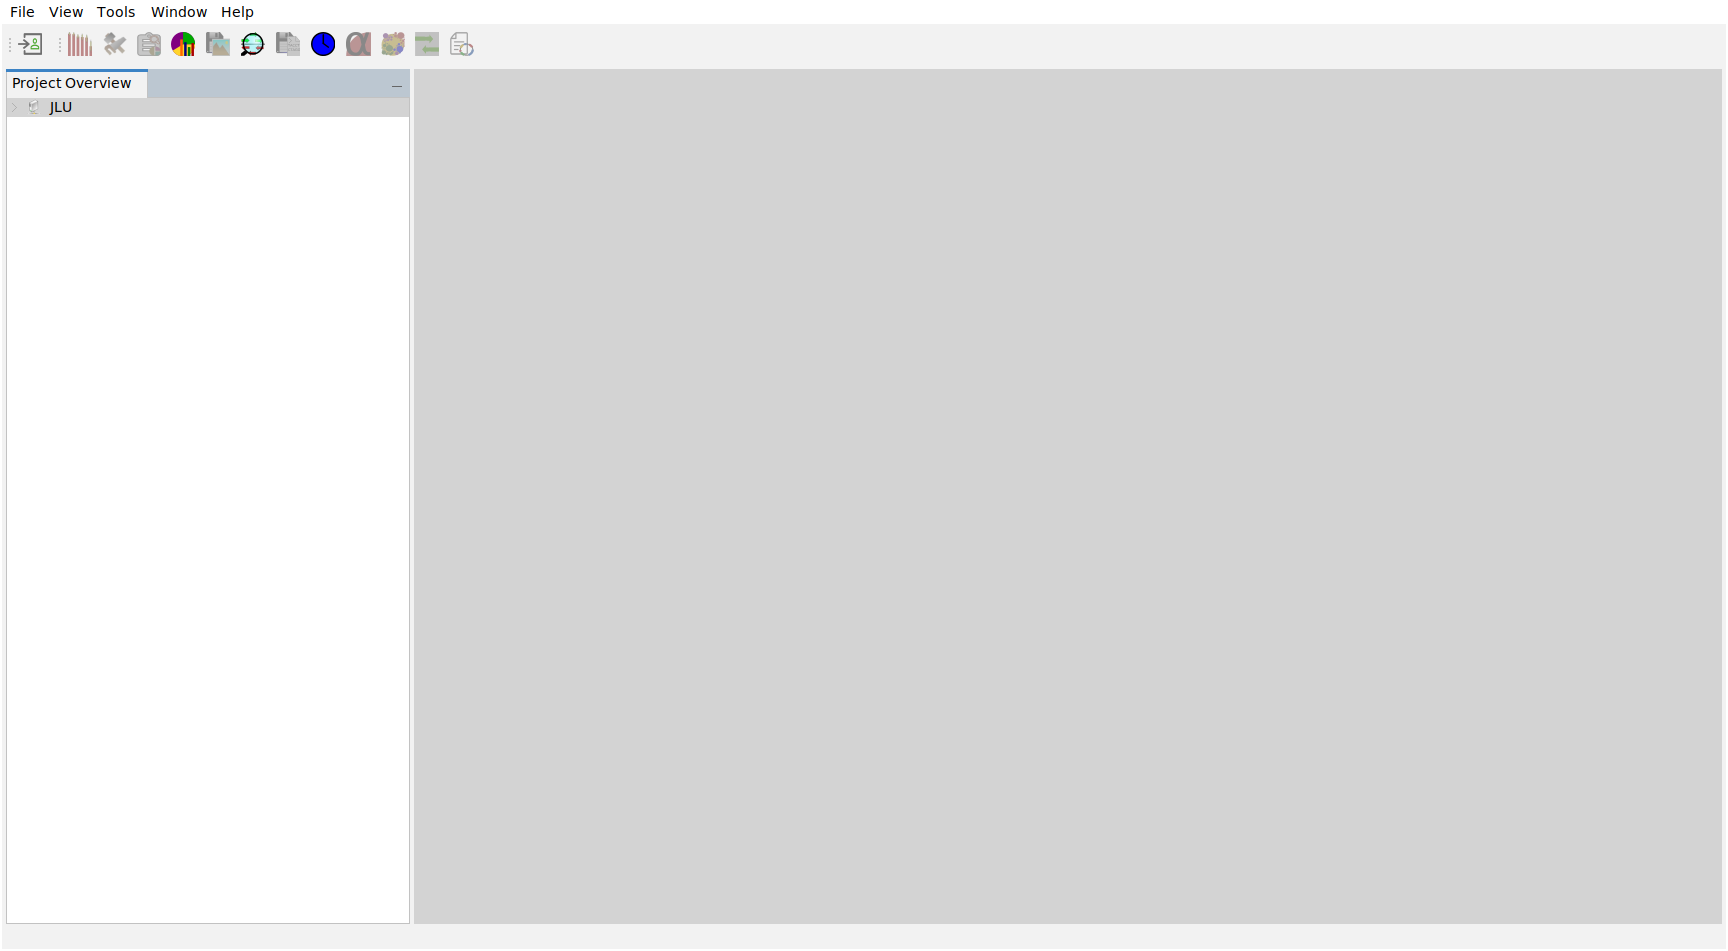
\includegraphics[width=\textwidth]{img/mgx/startup}
\caption[MGX client]{Screenshot of the client application right after startup.}
\label{startup}
\end{figure}

After installation, the MGX application is already preconfigured to connect to the 
MGX server instance hosted at CeBiTec, Bielefeld University. In case a different MGX server
should be used, the default server can be changed choosing Tools $\rightarrow$ Options from the menu
and navigating to the MGX server tab (\ref{config-site}). While the site name can be freely
chosen by the user, the server URL has to be entered as provided by the site administrators.

\begin{figure}[H]
\centering
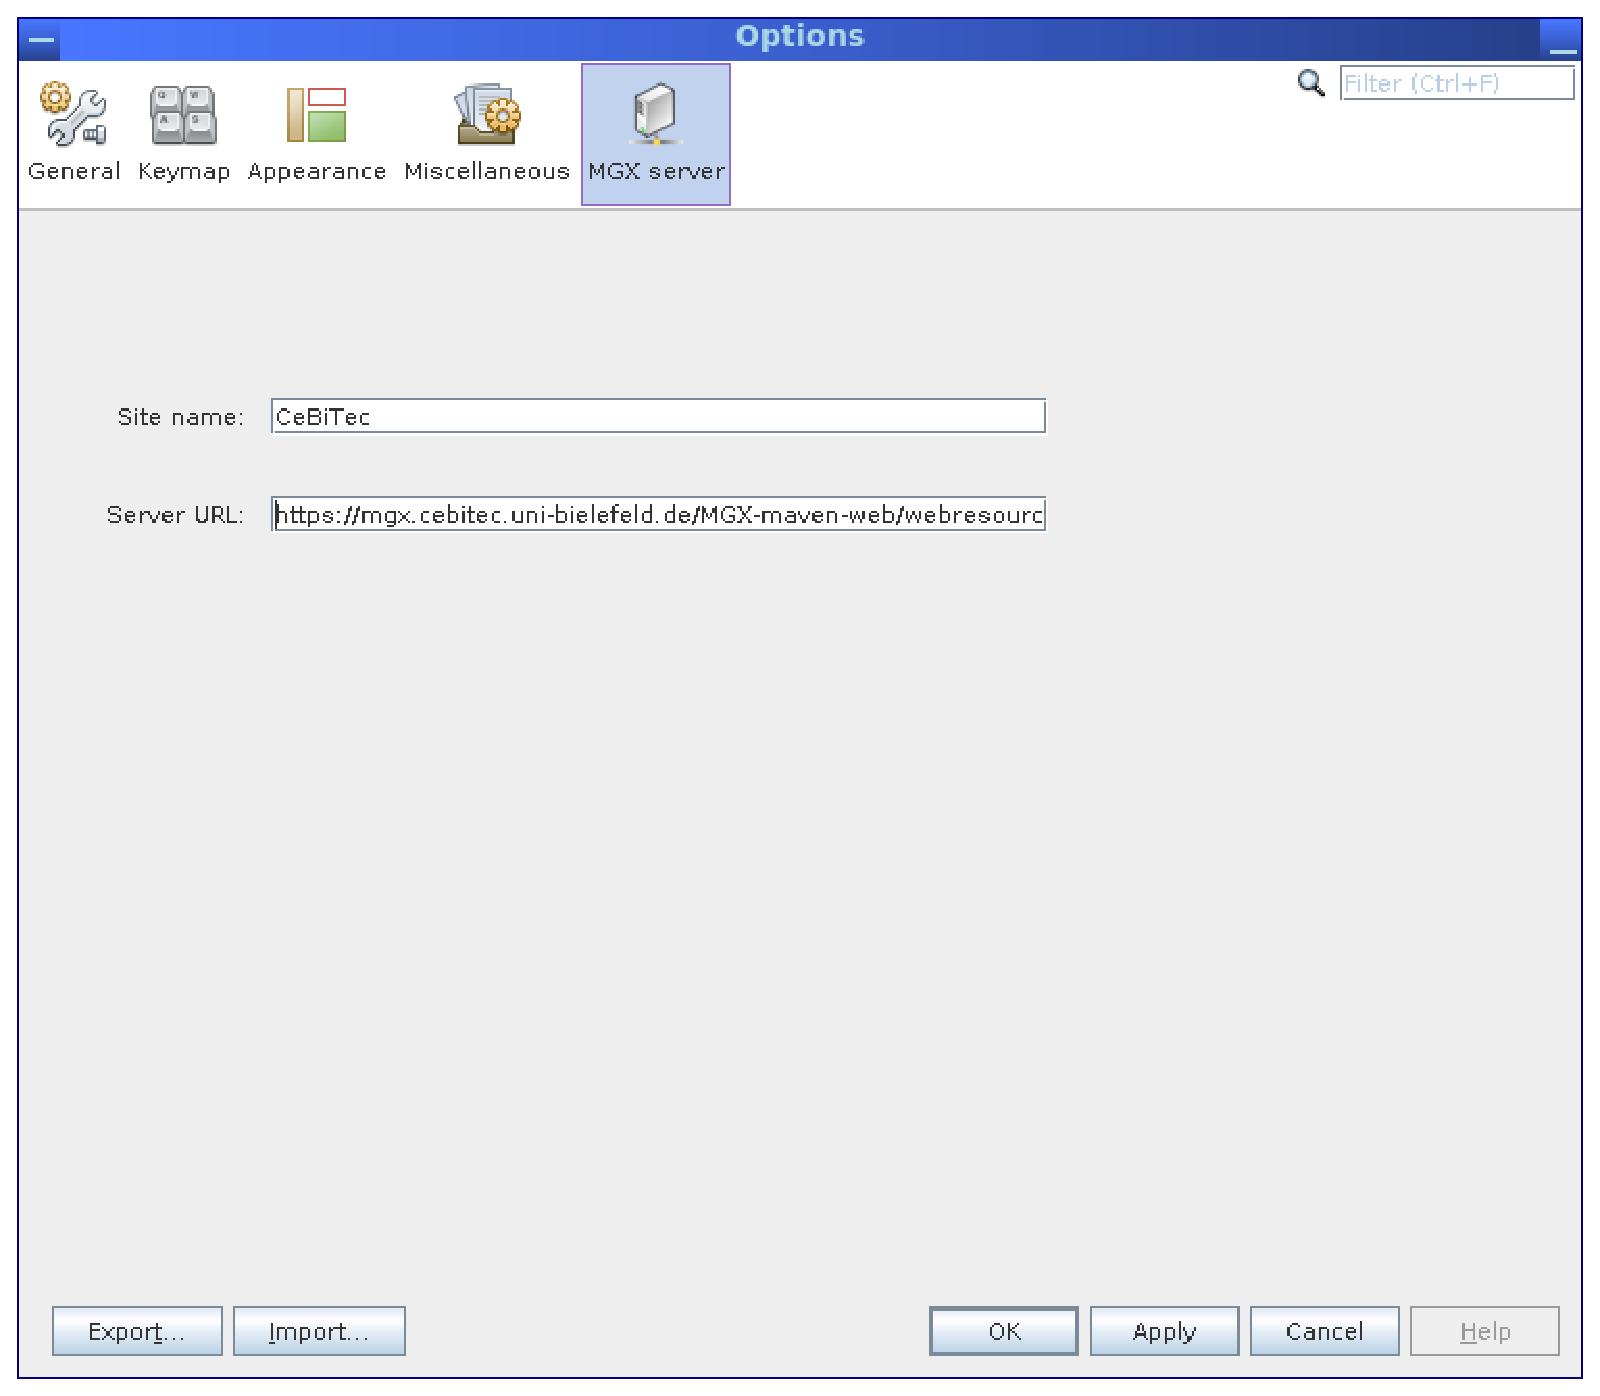
\includegraphics[width=.8\textwidth]{img/mgx/config-site}
\caption[Server configuration]{A different default server instance can optionally be configured in the MGX 
server tab, which is available from the Tools $\rightarrow$ Options menu.}
\label{config-site}
\end{figure}


\begin{figure}[H]
\centering
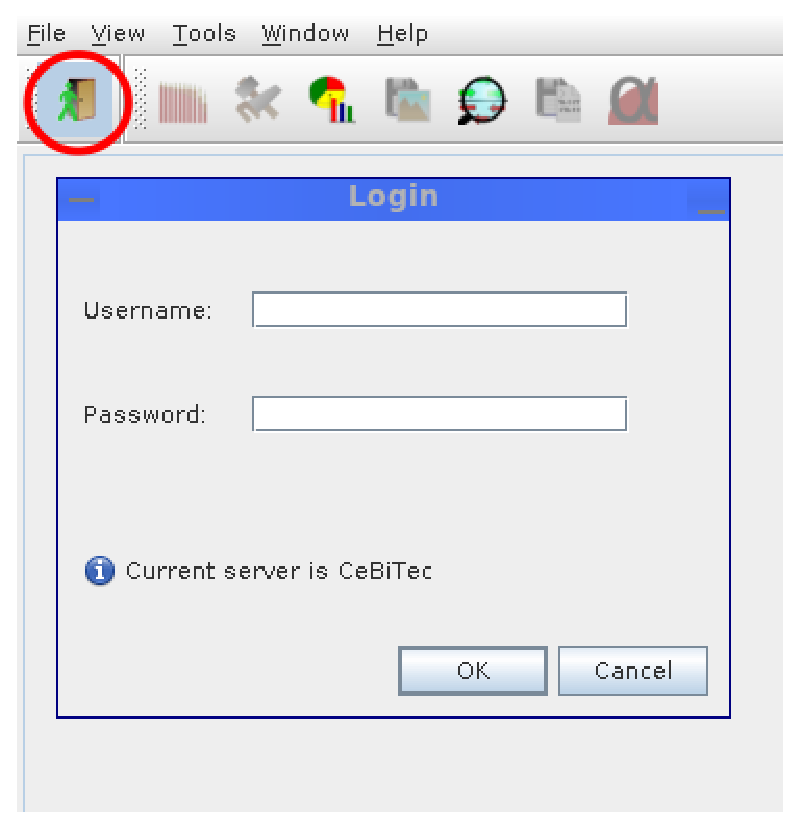
\includegraphics[width=.6\textwidth]{img/mgx/login}
\caption[Login screen]{The first button in the menu toolbar will bring up the login dialog, allowing to connect to the configured server; the login screen also reflects the name of the current server.}
\label{login-screen}
\end{figure}

All communication between the MGX user interface and the MGX server is encrypted using
the standardized SSL (Secure Sockets Layer) protocol, ensuring confidentiality of 
unpublished data and protecting the integrity of login credentials.
%\section{Browsing and exploring MGX projects}
After successfully logging in, a new window is automatically opened. The MGX Explorer window
lists all available projects a user is allowed to access, including both public as well as
private projects. Projects are easily opened or closed by simply expanding the corresponding
nodes in the Project Explorer window (\ref{projects}).\\

\begin{figure}[H]
\centering
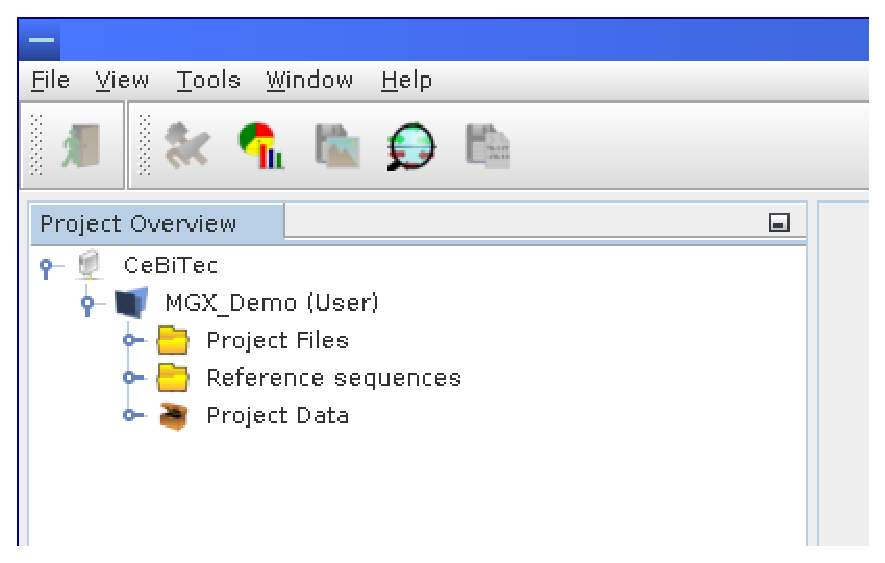
\includegraphics[width=.8\textwidth]{img/mgx/projects}
\caption[Project Explorer]{After successful login, the Project Explorer component will automatically open,
showing a list of MGX projects available to the current user. Shown is just one project, MGX\_Demo, with
``User'' access level indicated behind the project name.}
\label{projects}
\end{figure}

\begin{figure}[H]
\centering
\includegraphics[width=.4\textwidth]{img/mgx/projstructure}
\caption[Project structure]{Divided into three different parts, a MGX projects offers
(from top to bottom) dedicated storage for files to be used by analysis pipelines, 
managed reference sequences (including annotation data, if available) and general
project data containing metadata as well as sequence datasets.}
\label{structure}
\end{figure}

Each project contains metagenome datasets as well as structured storage (\ref{structure}), where user-provided
databases can be uploaded to be used in custom analysis pipelines (Chapter \ref{custom}).

\section{Creating a new habitat}

New habitats are defined choosing ''Add habitat'' (\ref{addhabitat}) from the context menu of the ''Project Data''
node. This will bring up a wizard allowing to select the corresponding geographical location as well as
specifying a habitats name and biome type (\ref{habwiz}). In a second step, an optional description for this
habitat may be entered, as well.

\begin{figure}[H]
\centering
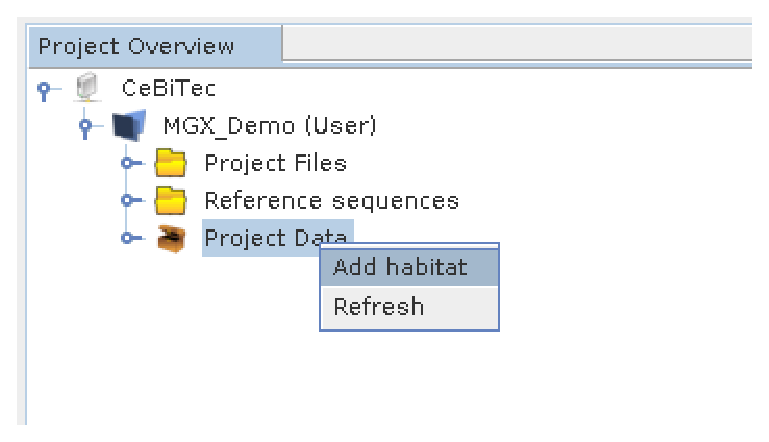
\includegraphics[width=.6\textwidth]{img/mgx/addhabitat}
\caption[Habitat creation]{A new habitat can be added selecting the appropriate entry from the context
menu of the ''Project Data'' node.}
\label{addhabitat}
\end{figure}

\begin{figure}[H]
\centering
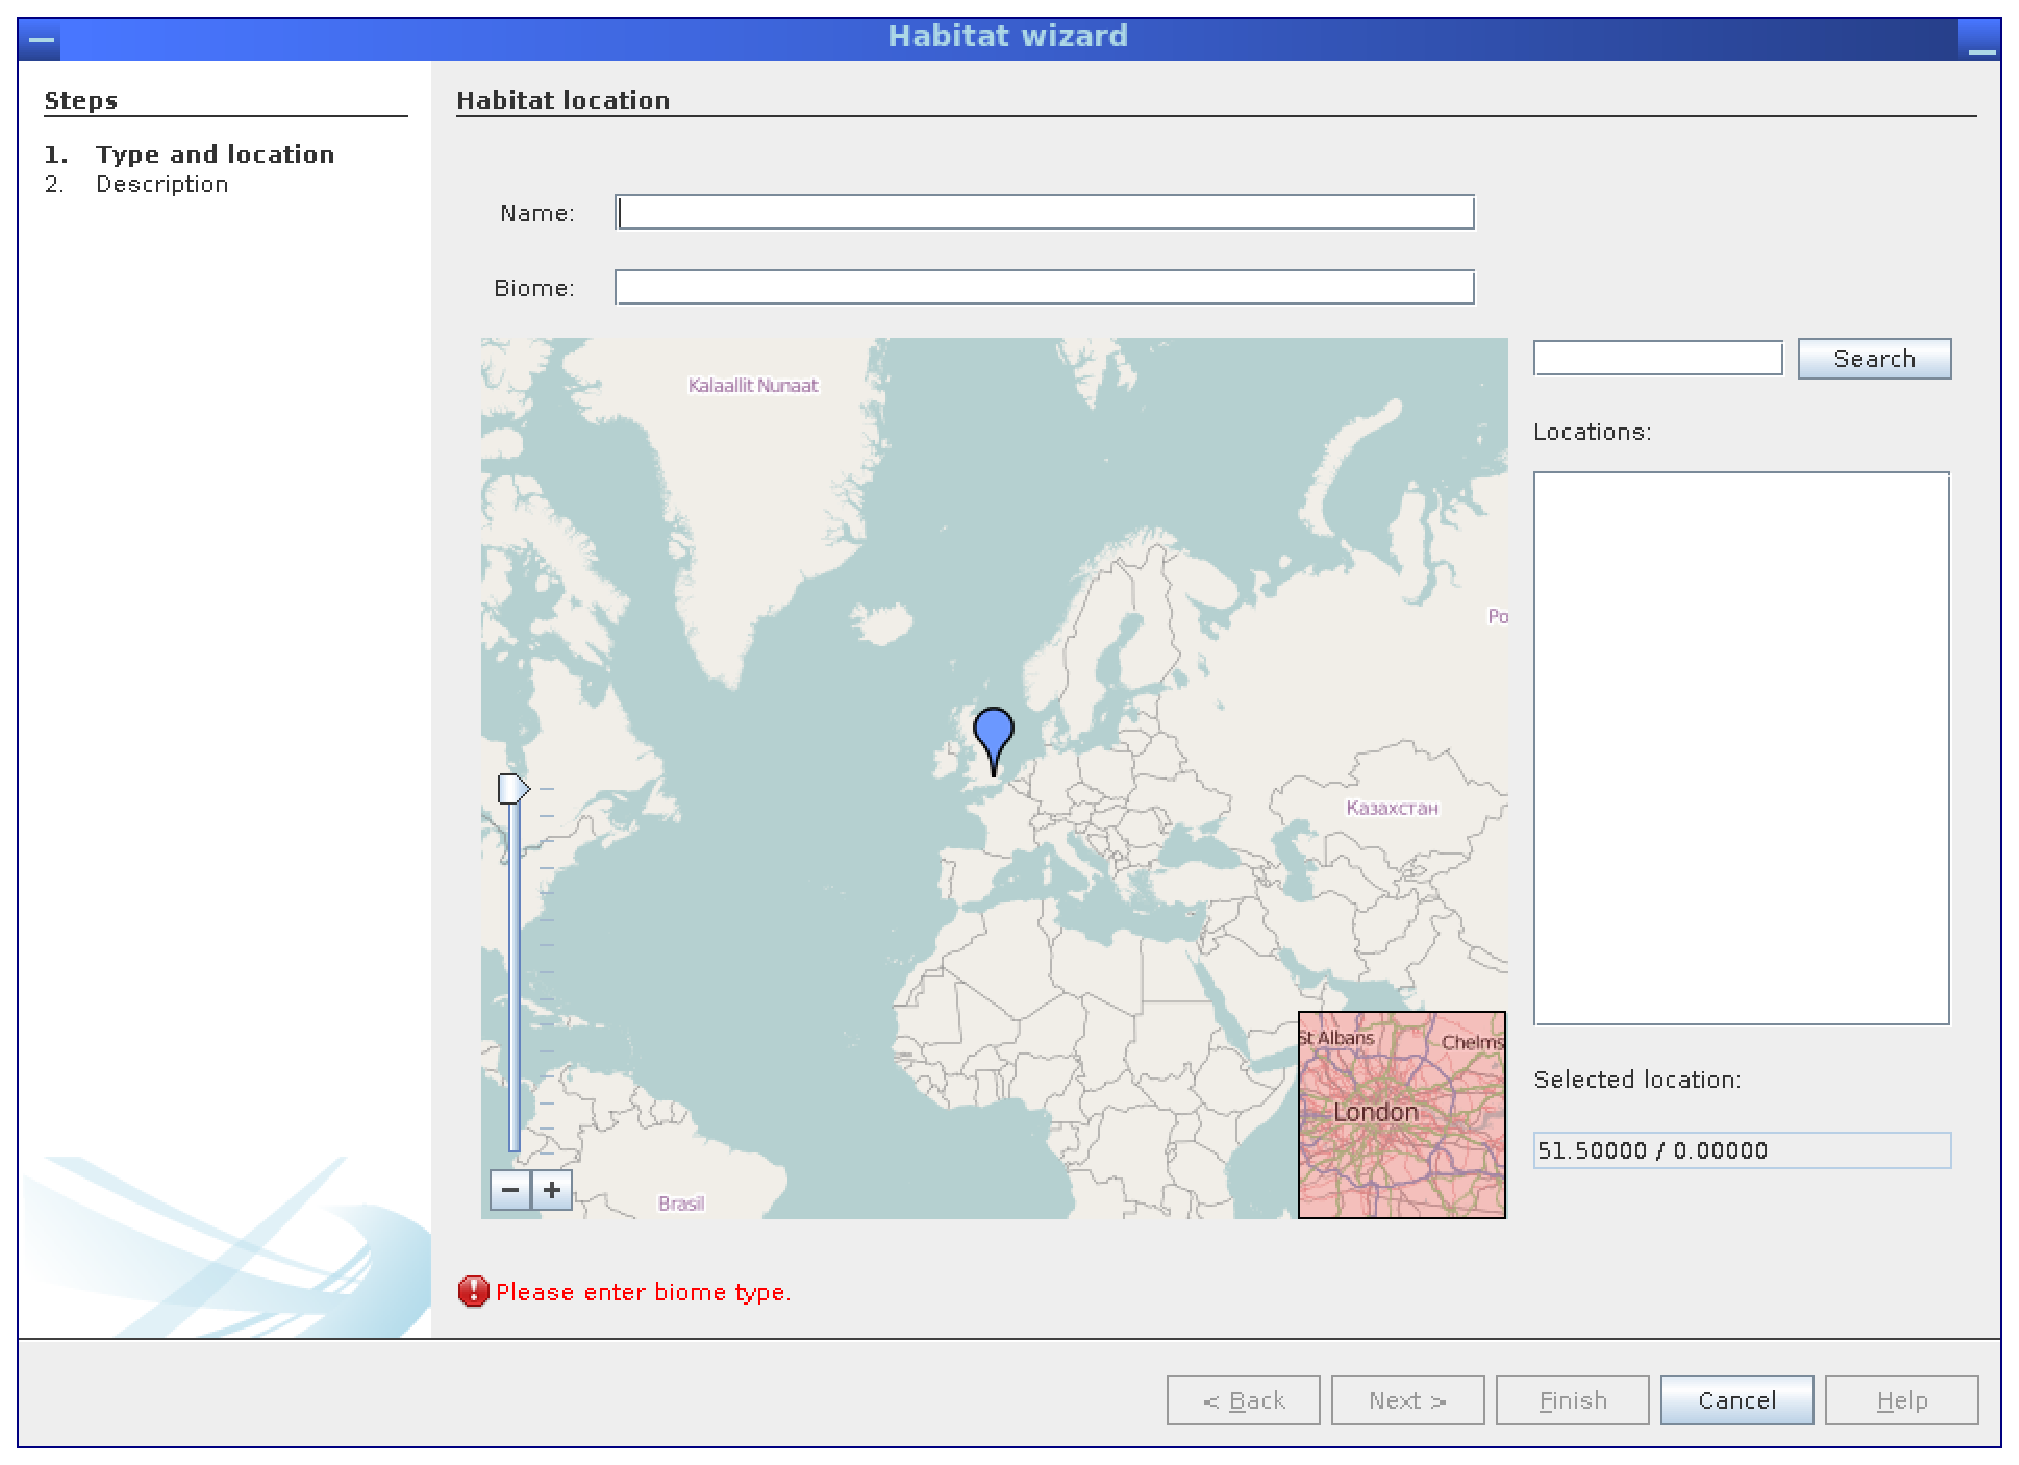
\includegraphics[width=.8\textwidth]{img/mgx/habwizard}
\caption[Habitat wizard]{The habitat wizard allows to define new habitats specifying their location, name and
biome type.}
\label{habwiz}
\end{figure}

\section{Creating new samples and DNA extracts}

Samples and DNA extracts are created in the same way as habitats, except that samples are defined for
habitats and DNA extracts are defined based on samples. Thus, the corresponding wizards are available
from the context menu of the ''Habitat'' and ''Sample'' nodes, respectively.

\begin{figure}[H]
\centering
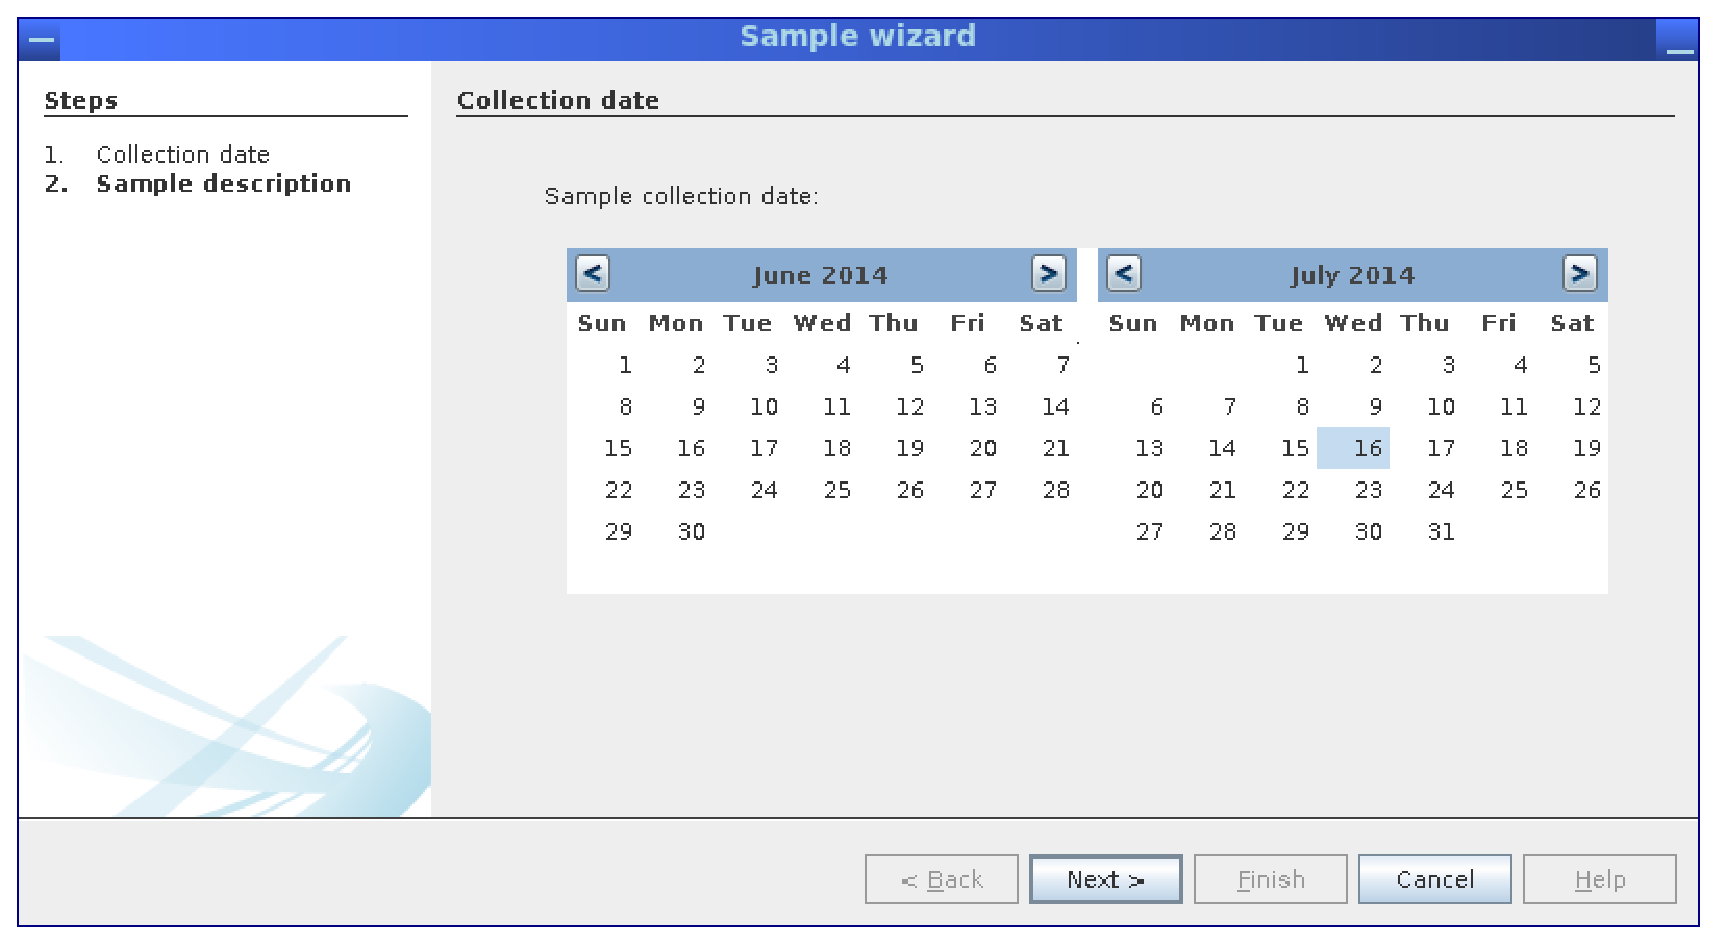
\includegraphics[width=.8\textwidth]{img/mgx/samplewiz1}
\caption[Sample wizard]{In the first step of the sample wizard, the sampling date is selected.}
\label{samplewiz1}
\end{figure}

\begin{figure}[H]
\centering
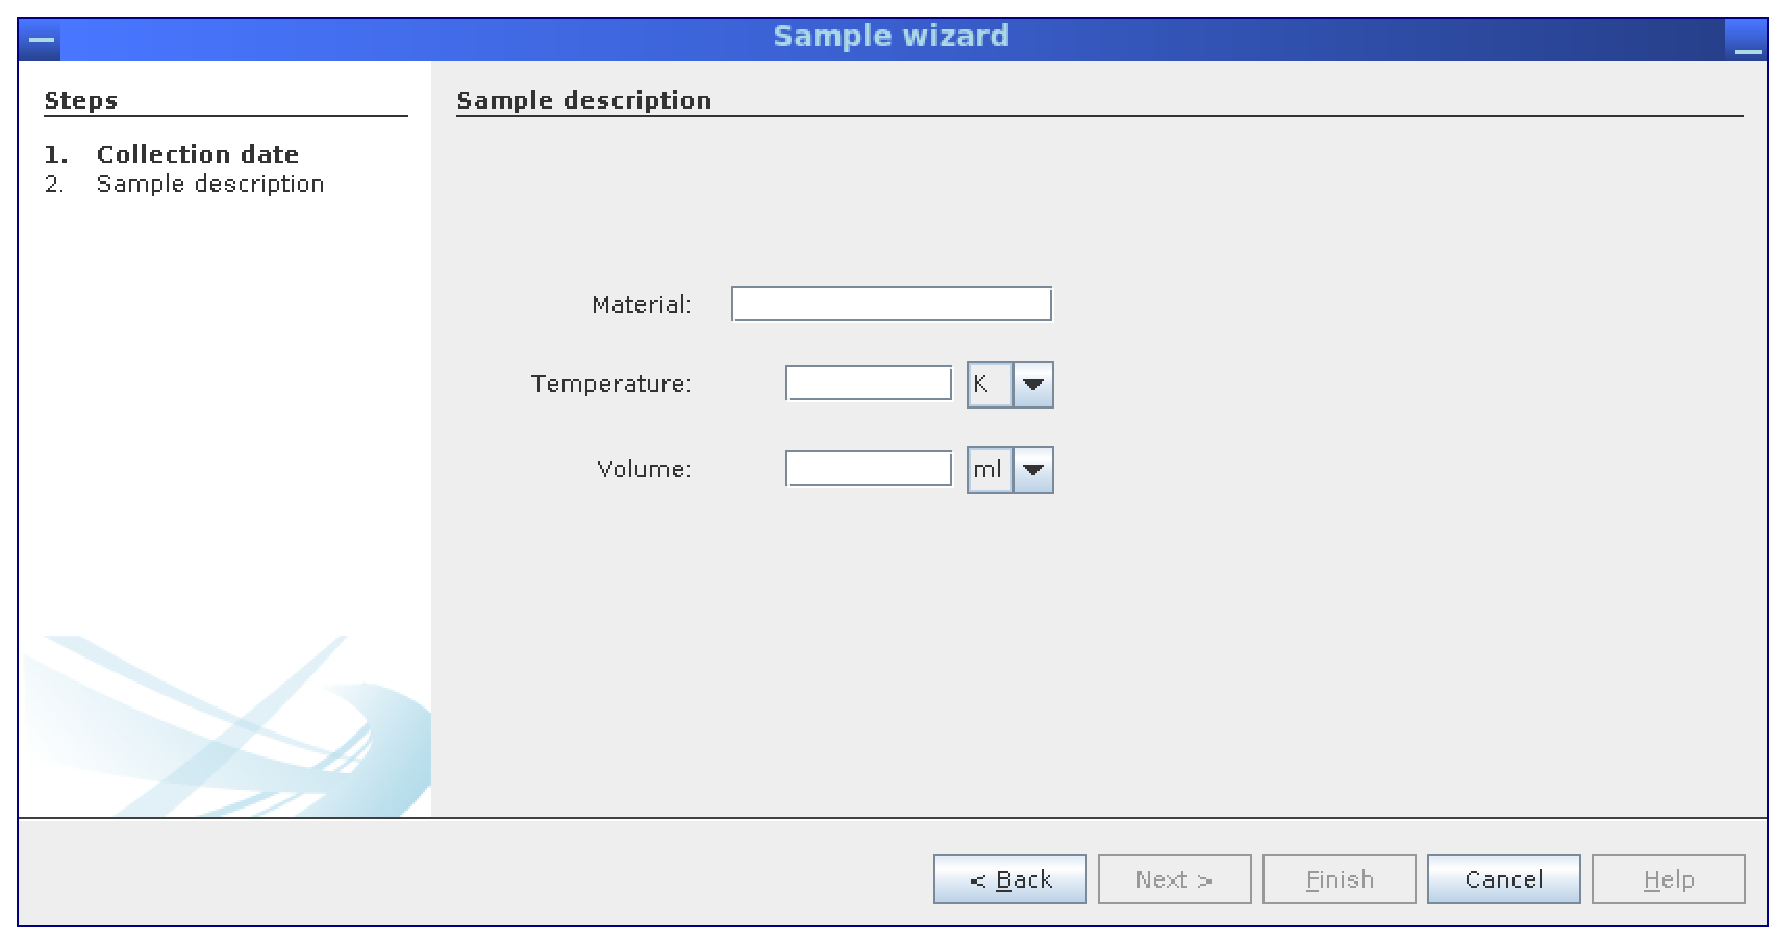
\includegraphics[width=.8\textwidth]{img/mgx/samplewiz2}
\caption[Sample wizard]{In the second step, the sampled material as well as temperature and sampled volume/weight
need to be entered.}
\label{samplewiz2}
\end{figure}

\begin{figure}[H]
\centering
\includegraphics[width=.8\textwidth]{img/mgx/extractwiz1}
\caption[DNA extract wizard]{The DNA extract wizard allows to specify the type of DNA extract (metagenome, 
metatranscriptome, amplicon) and protocols used to extract the DNA.}
\label{extractwiz1}
\end{figure}

\begin{figure}[H]
\centering
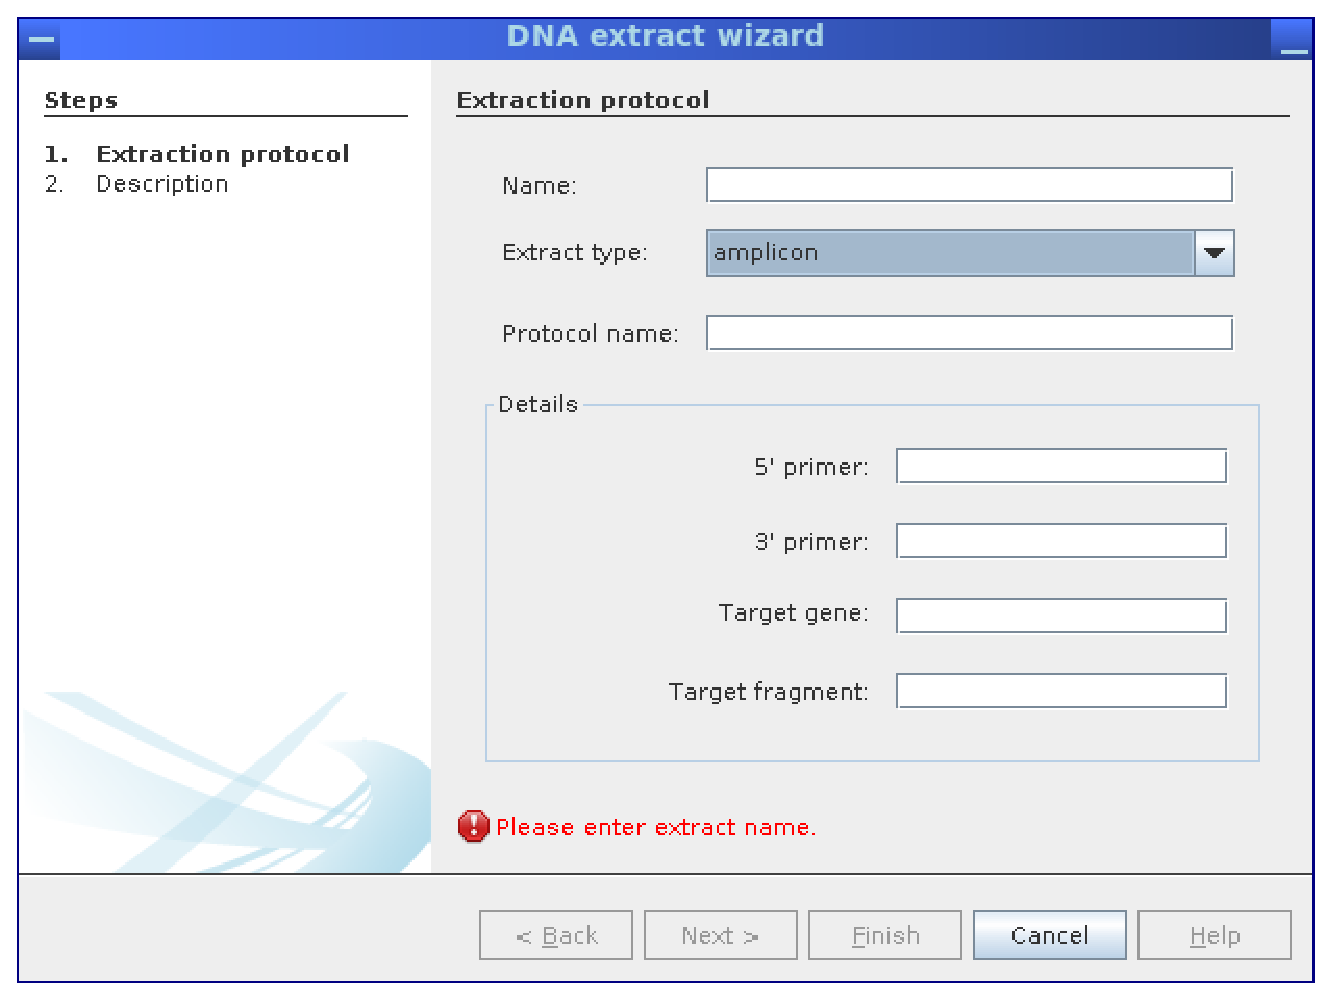
\includegraphics[width=.8\textwidth]{img/mgx/extractwiz2}
\caption[DNA extract wizard]{Depending on DNA extract type, additional data can be provided; for amplicons, primer
names and the corresponding target gene (fragment) can be entered, for metatranscriptomes, the type of RNA depletion
methods can be selected.}
\label{extractwiz2}
\end{figure}

\section{Importing sequence data}

\begin{figure}[H]
\centering
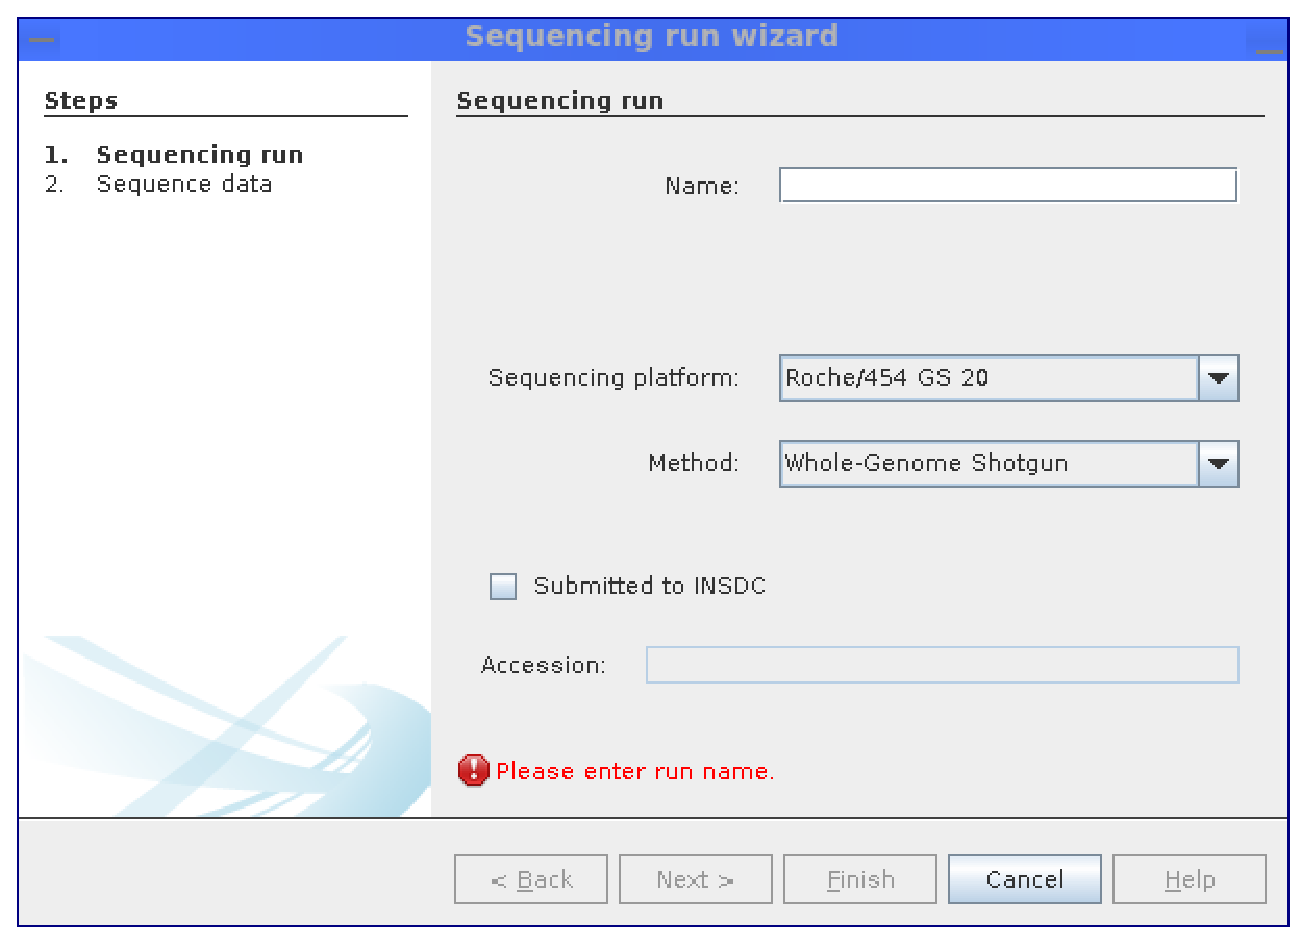
\includegraphics[width=.8\textwidth]{img/mgx/runwiz1}
\caption[Sequence import]{Before sequence data can be uploaded, the employed sequencing platform and technology have 
to be specified; for data already submitted to or obtained from public INSDC repositories (e.g. NCBI, EBI, DDBJ), the
corresponding accession number can be stored, as well.}
\label{dnawiz1}
\end{figure}

\begin{figure}[H]
\centering
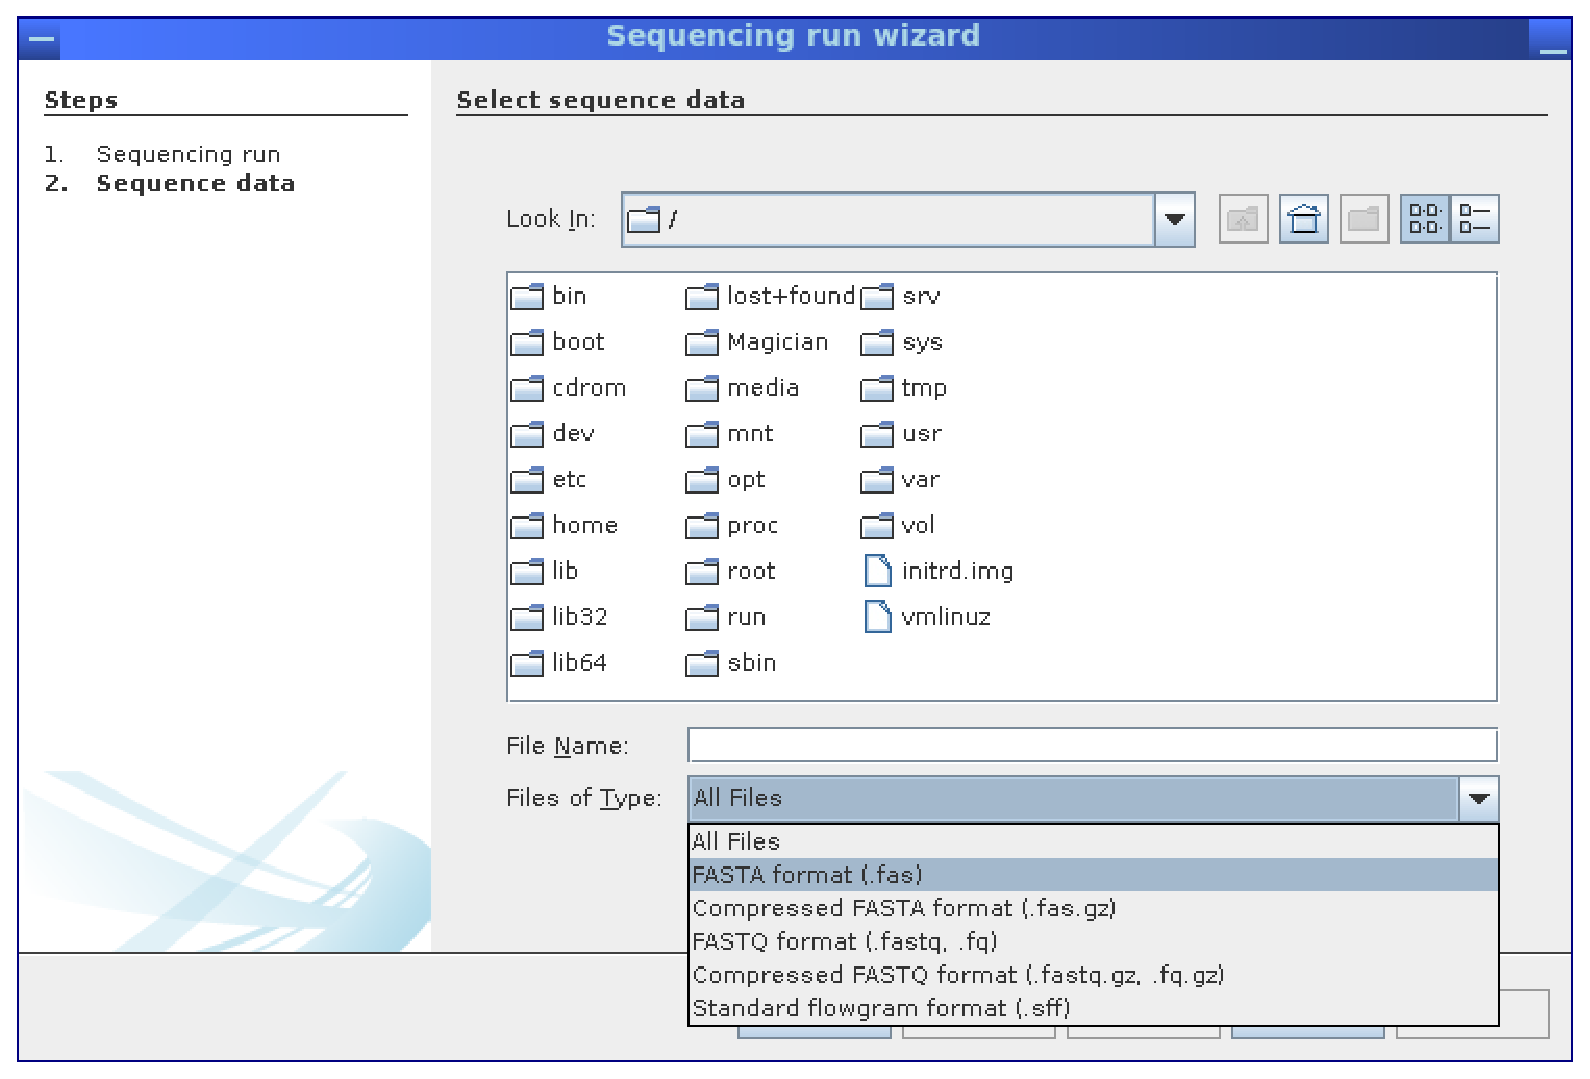
\includegraphics[width=.8\textwidth]{img/mgx/runwiz2}
\caption[Sequence import]{Finally, the file containing the sequence data is selected; MGX supports all commonly used
file formats such as FASTA, FASTQ, or SFF.}
\label{dnawiz2}
\end{figure}

\section{Quality control}

\begin{figure}[H]
\centering
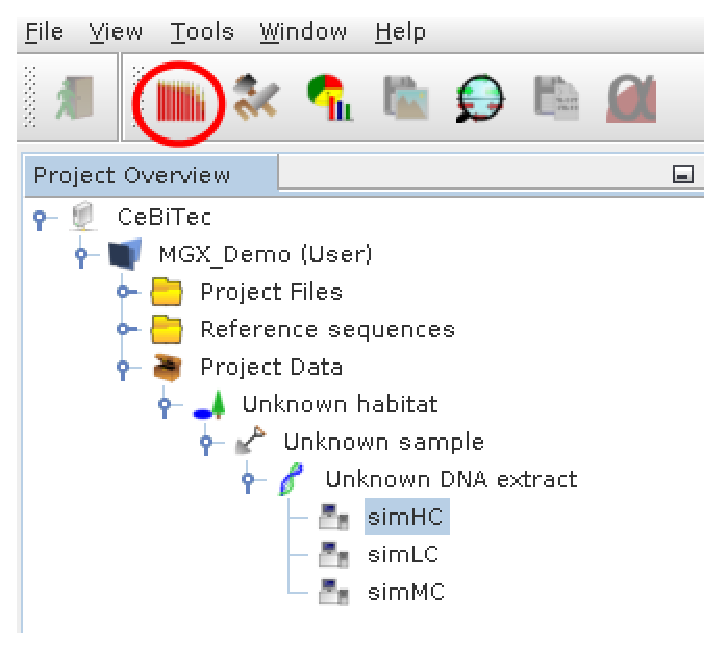
\includegraphics[width=.6\textwidth]{img/mgx/QCopen}
\caption[Quality control]{After selecting a sequencing run object, the Quality Control component can be opened
from its menubar icon (red circle).}
\label{qcopen}
\end{figure}

After sequence import, Quality control reports generated within MGX should be inspected (\ref{qcopen}) before proceding with data analysis.
MGX currently offers three types of QC reports: Distribution of GC content, sequence length
and nucleotide distribution within the DNA sequences. Those can be used to evaluate overall
sequence data quality and check for possible signs of contamination.
For demonstration purposes, data shown relates to the artificial \textbf{simHC} metagenome dataset created by the
FAMeS \cite{SIMMETA} project. The actual sequence data is publicly available and can be obtained from
the FAMeS web site (\url{http://fames.jgi-psf.org/Retrieve_data.html}).

\begin{figure}[H]
\centering
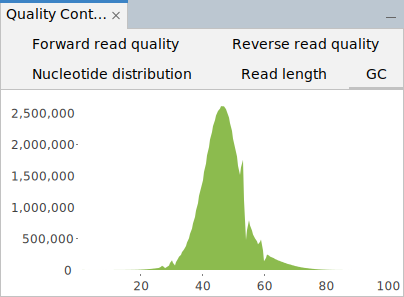
\includegraphics[width=.6\textwidth]{img/mgx/QCgc}
\caption[Quality control]{GC distribution of the simHC dataset.}
\label{qc1}
\end{figure}

\begin{figure}[H]
\centering
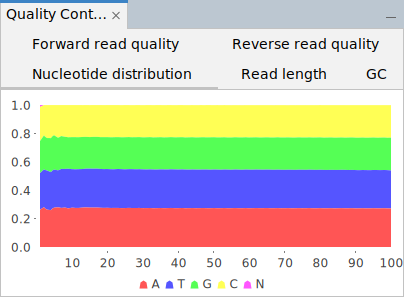
\includegraphics[width=.6\textwidth]{img/mgx/QCnuc}
\caption[Quality control]{Nucleotide distribution of the simHC dataset. A high fraction of uncalled bases
is apparent from the chart.}
\label{qc2}
\end{figure}

\begin{figure}[H]
\centering
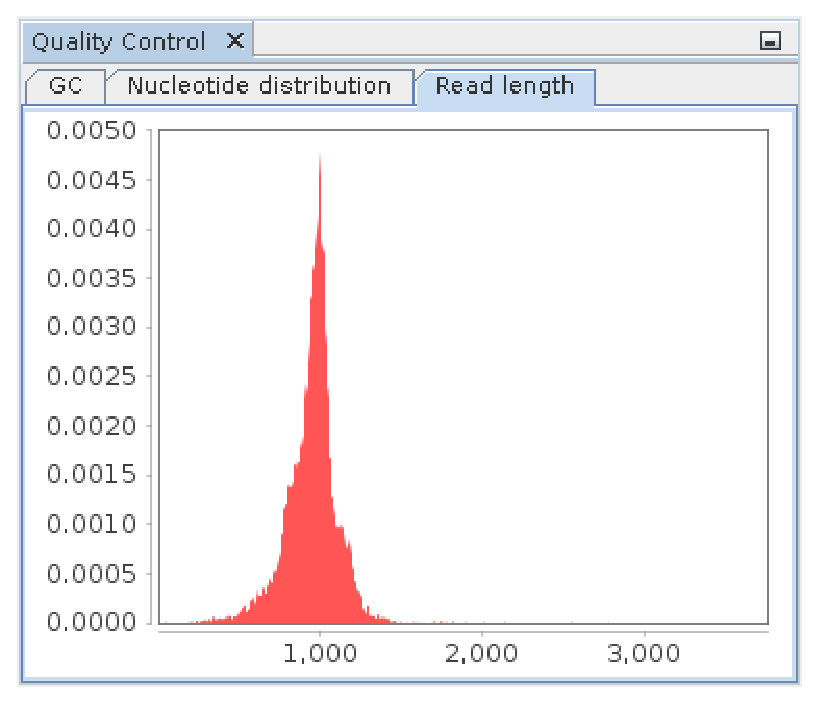
\includegraphics[width=.6\textwidth]{img/mgx/QCreadlen}
\caption[Quality control]{Read length distribution of the simHC dataset. }
\label{qc3}
\end{figure}

\begin{figure}[H]
        \centering
        \begin{subfigure}[b]{0.3\textwidth}
                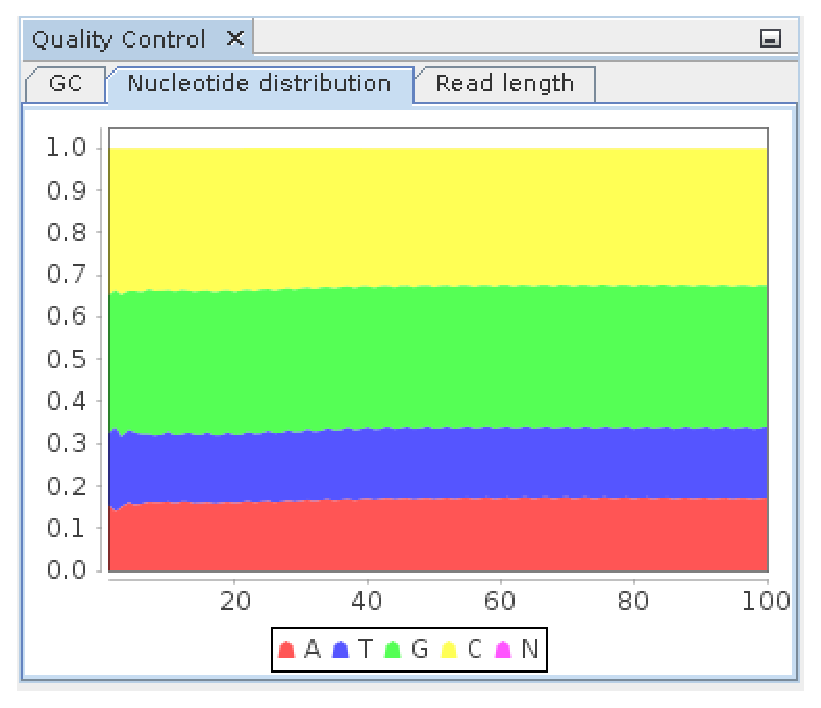
\includegraphics[width=\textwidth]{img/mgx/highGCnucl}
                \caption{High-GC (65\%) data}
        \end{subfigure}%
        \begin{subfigure}[b]{0.3\textwidth}
                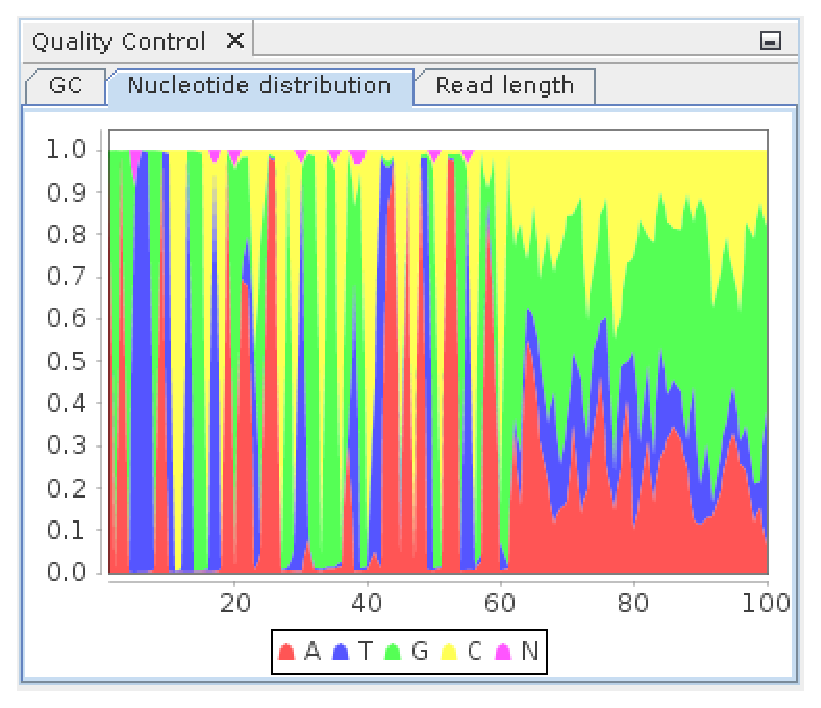
\includegraphics[width=\textwidth]{img/mgx/ampliconNucl}
                \caption{Amplicon data}
        \end{subfigure}
        \begin{subfigure}[b]{0.3\textwidth}
                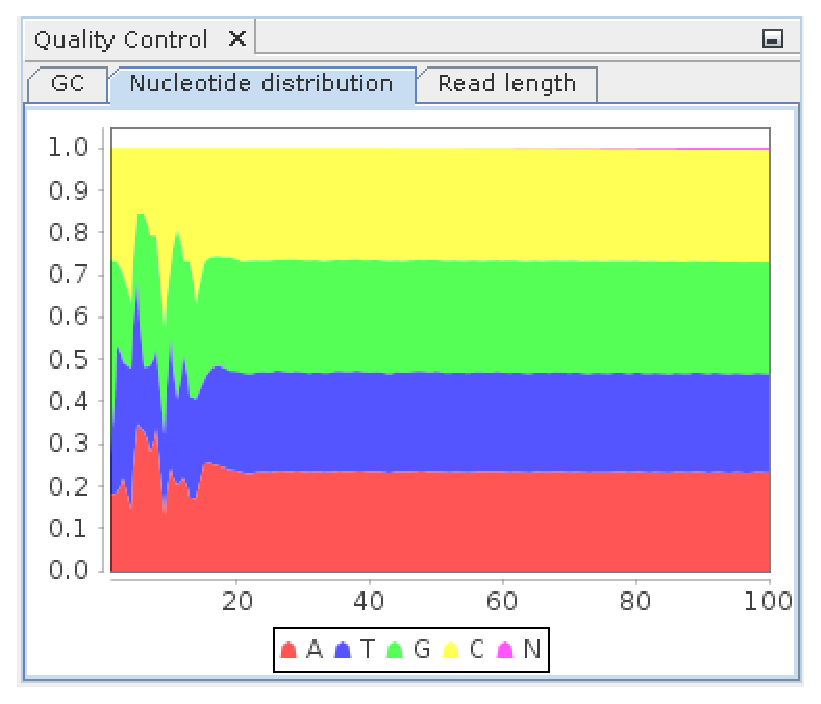
\includegraphics[width=\textwidth]{img/mgx/adapterNucl}
                \caption{Adapter residue}
        \end{subfigure}
        \caption{Nucleotide distribution examples.}
  \label{qc4}
\end{figure}

Depending on the kind of sequence data, different patterns might emerge (\ref{qc4}),
which might or might not warrant any further action. While small amounts of e.g. 
adapter residue are sometimes encountered and might be considered acceptable, it is up to the
individual researcher to check back with their sequencing provider and ask for
adapter sequences to execute additional trimming.

\section{Defining and executing analysis jobs}

\subsection{Selecting an analysis pipeline}

\begin{figure}[H]
\centering
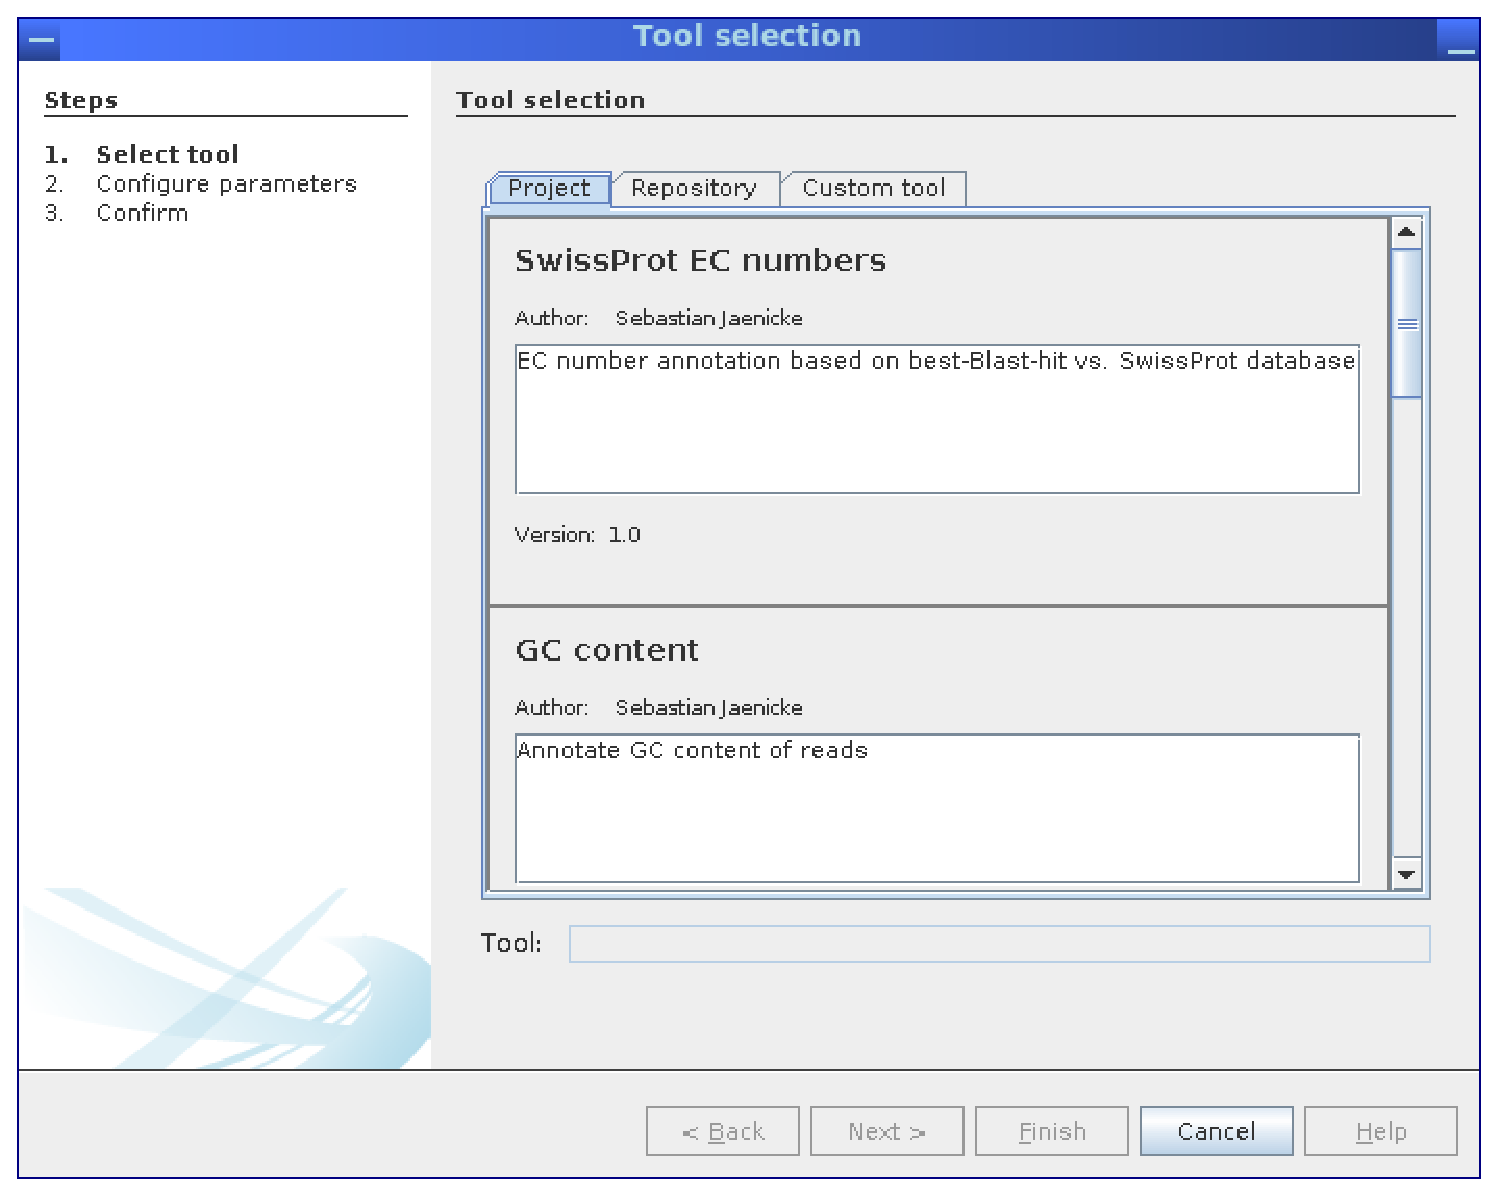
\includegraphics[width=.8\textwidth]{img/mgx/analysiswiz1}
\caption[Analysis selection]{Analysis pipelines can be selected from the corresponding
MGX project itself, from the repository of public pipelines provided by the server, or,
a custom workflow can be uploaded and executed.}
\label{anawiz1}
\end{figure}

All analysis pipelines can be started from the context menu of the metagenome dataset to be analyzed, provided
the user has been granted at least ``User'' level access. First,
the user can choose the desired pipeline from the project itself, from the pipeline repository hosted on the
MGX server, or upload an own pipeline implementation (\ref{anawiz1}). Subsequently, analysis parameters
can be reviewed and adapted (\ref{anawiz2}) before submitting an analysis.

\begin{figure}[H]
\centering
\includegraphics[width=.8\textwidth]{img/mgx/analysiswiz2}
\caption[Analysis parameters]{The wizard allows to inspect and adapt parameters for the selected pipeline. The actual
number of steps depends on the number of parameters available for customization.}
\label{anawiz2}
\end{figure}

\begin{figure}[H]
\centering
\includegraphics[width=.8\textwidth]{img/mgx/analysiswiz3}
\caption[Parameter overview]{Before executing an analysis pipeline, a final overview of all parameters is shown. Once
confirmed, the pipeline is submitted and scheduled for execution on the MGX server. Here, the selected pipeline has
only one single parameter.}
\label{anawiz3}
\end{figure}

\subsection{Monitoring job progress}

\begin{figure}[H]
\centering
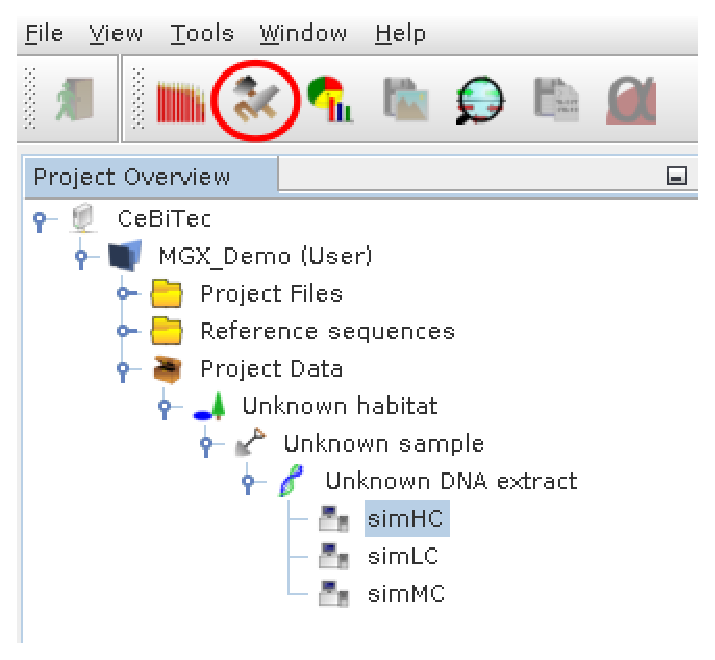
\includegraphics[width=.6\textwidth]{img/mgx/JobMonOpen}
\caption[Job monitor]{The Job Monitor component can be opened using its icon in the toolbar.}
\label{jobmon1}
\end{figure}

\begin{figure}[H]
\centering
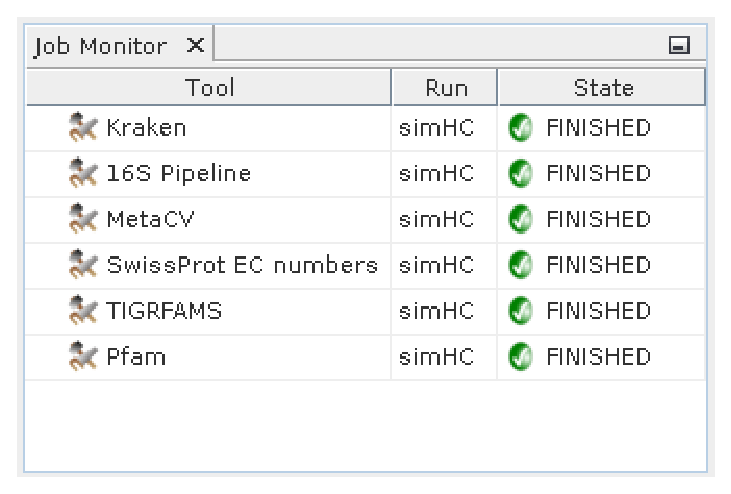
\includegraphics[width=.6\textwidth]{img/mgx/JobMon}
\caption[Job monitor]{The Job Monitor provides an overview of job states. Depending on context, all jobs
within a MGX project or only jobs for a single dataset will be displayed.}
\label{jobmon2}
\end{figure}

The Job Monitor component is provided to inspect the state of jobs present within a MGX project.
It can be opened from the toolbar (\ref{jobmon1} )and will display the state of jobs scheduled for execution,
currently running or already finished (\ref{jobmon2}). In addition, it can also be used to delete jobs and
corresponding analysis results when no longer needed. Depending on the selected item in the
Project Explorer, the Job Monitor will by default display all jobs within a project; if a single
sequencing run is selected, only jobs for this dataset will be shown.

\section{Visualization of results}

\begin{figure}[H]
\centering
\includegraphics[width=.6\textwidth]{img/mgx/VizOpen}
\caption[Visualization]{Icon for the visualization module.}
\label{viz1}
\end{figure}

\begin{figure}[H]
\centering
\includegraphics[width=.8\textwidth]{img/mgx/VizComponent}
\caption[Visualization components]{Components of the visualization module. The bottom window is
used to create and define groups, while the top window allows to select result and visualization
type, customize options and display the final chart.}
\label{viz2}
\end{figure}

The visualization component actually consists of two separate windows (\ref{viz2}). The Group
Window is located at the bottom and used to create, name and define groups used for data display.
Sequencing runs can be added to individual groups using \textit{Drag and Drop}. While any
sequencing run can be present in several groups at the same time, it is not possible to add
it to a group more than once. Groups may be assigned a name, their display color can be chosen
by the user, and they may be temporarily excluded from display.\\
The main visualization window is shown at the top; once sequencing runs are added or changed, 
the type of analysis result to be shown can be chosen on the top right. Afterwards, the desired
visualization type is selected and may be customized, as well.

\begin{figure}[H]
\centering
\includegraphics[width=\textwidth]{img/mgx/VizDemo}
\caption[Visualization example]{Visualization example displaying a bar chart for two groups.}
\label{viz3}
\end{figure}

Figure \ref{viz3} shows a simple visualization example. Two groups were defined containing the simLC and simMC metagenomes
in the first and the simHC metagenome in the second group. The main visualization window shows a bar chart
generated for these groups based on assigned EC numbers. To account for differences in dataset size, both
groups are normalized to fractions.

\begin{figure}[H]
\centering
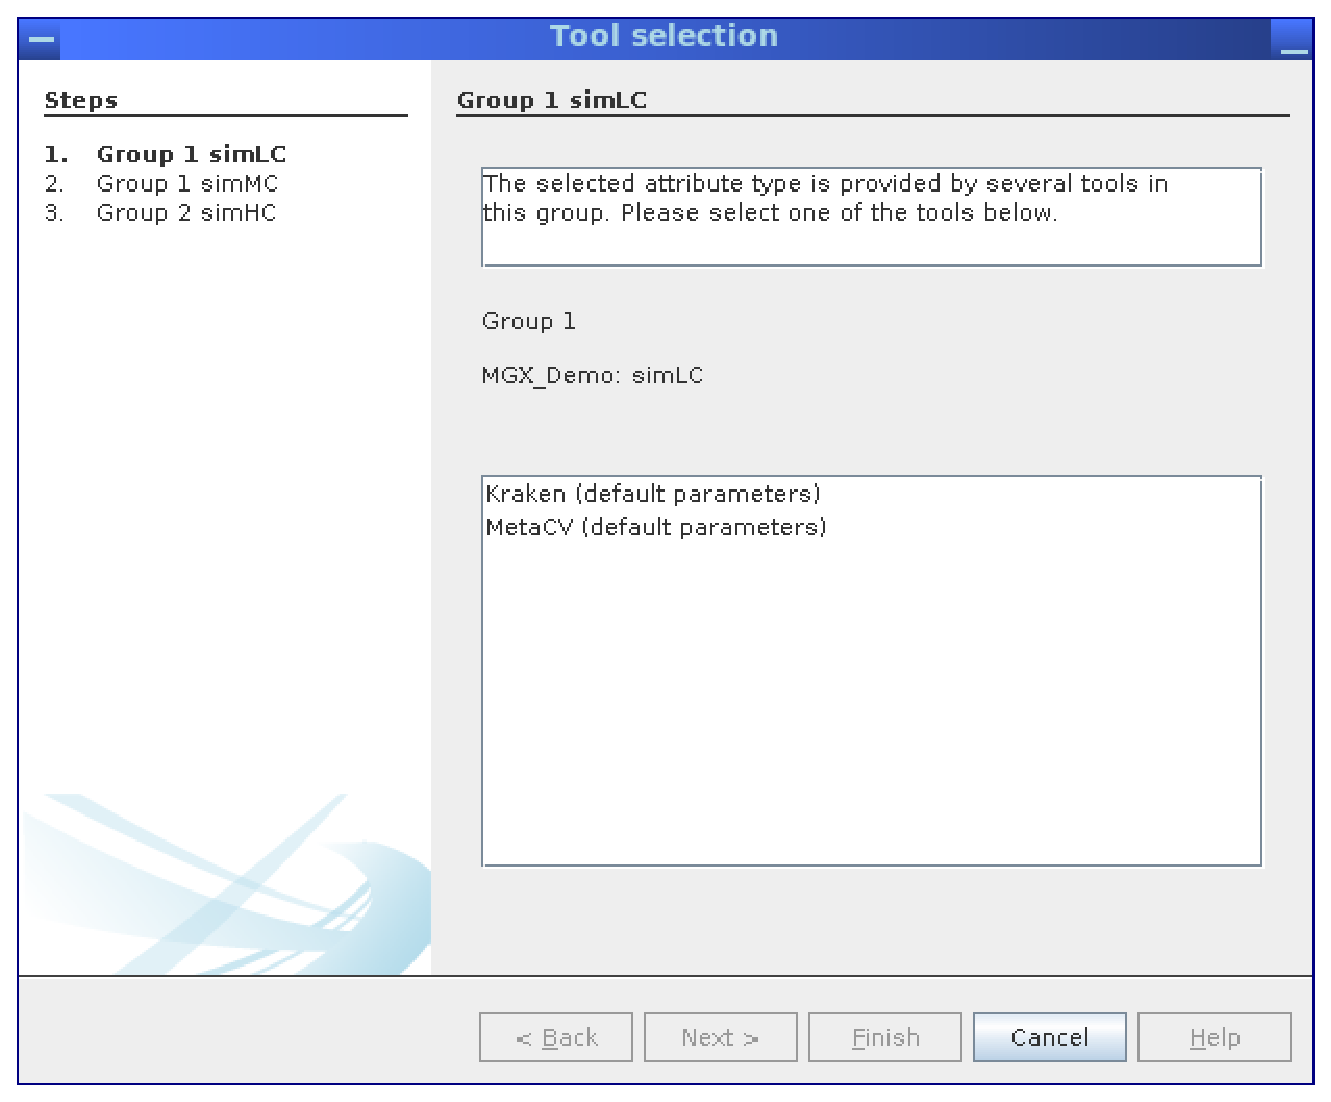
\includegraphics[width=.8\textwidth]{img/mgx/ConflictResolver}
\caption[Job selection]{In case a result is provided by more than one job, e.g. different taxonomic assignment methods,
a dialog allows to select between jobs. In this example, taxonomic assignments are provided by MGX pipelines employing Kraken \cite{KRAKEN}
as well as MetaCV \cite{METACV}.}
\label{viz4}
\end{figure}

Whenever a selected result type is provided by more than one analysis job, an interactive dialog allows the user to
review possible jobs and select one (\ref{viz4}). This scenario will occur when a tool is executed several 
times with different parameters, or when different taxonomic classifiers were used to analyse a dataset.

\subsection{Exporting sequences}

\begin{figure}[H]
\centering
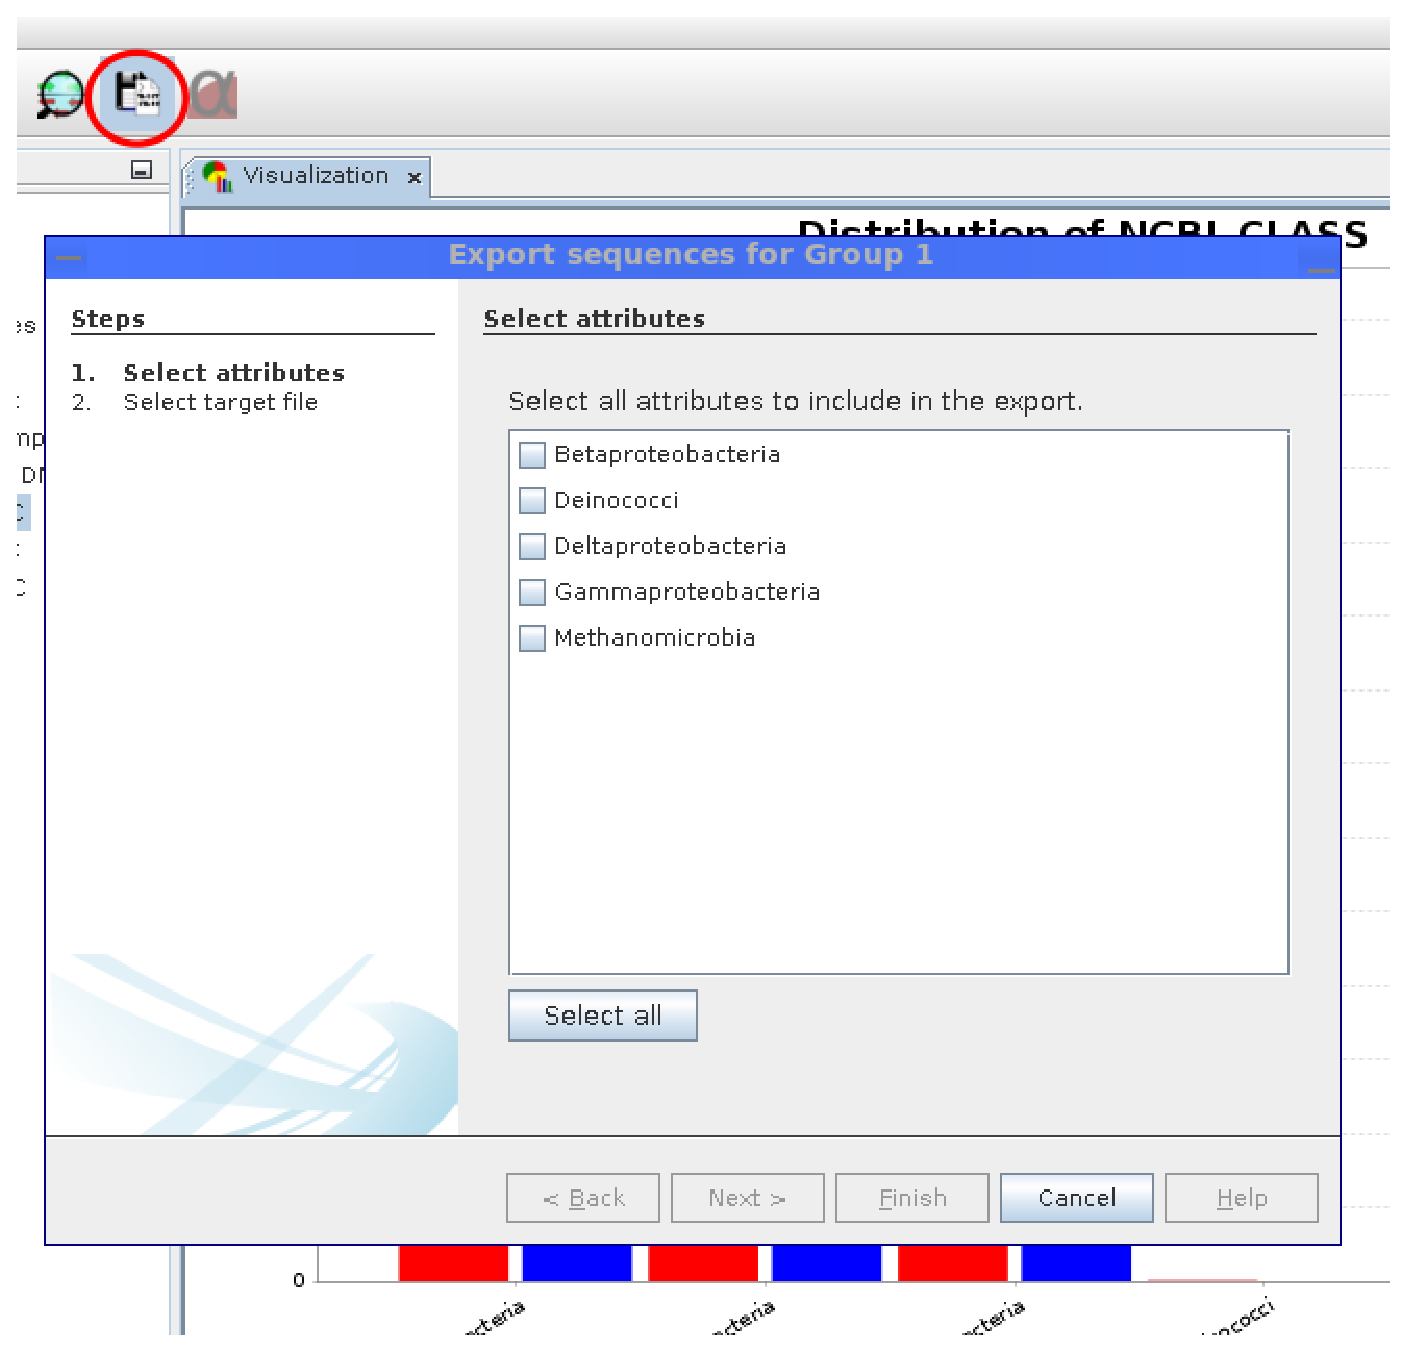
\includegraphics[width=.8\textwidth]{img/mgx/SeqExport}
\caption[Exporting sequences]{Sequences can be exported for each group individually. The user can freely choose
which attributes should be included.}
\label{seqexp}
\end{figure}

The sequence export wizard allows to export sequences conditionally based on analysis results. For each
visualization group, it is possible to choose the attributes for which sequences should be obtained (\ref{seqexp}).
Sequences are subsequently downloaded from the MGX server and saved in FASTA format files for each group.


\subsection{Biodiversity indices}

\begin{figure}[H]
\centering
\includegraphics[width=\textwidth]{img/mgx/BioDiversity}
\caption[Biodiversity]{Biodiversity indices (bottom left) such as ACE or Shannon are computed for the currently
selected visualization group.}
\label{biodiv}
\end{figure}

The visualization module features another component used to display commonly used biodiversity indices, such as
the ACE, Shannon \cite{SHANNON}, Chao1 \cite{DIVERSITY} and Simpson \cite{SIMPSON} indices. The component will automatically show the index values for the
currently selected visualization group based on the chosen attribute type (\ref{biodiv}).


\section{Uploading own files}

For each project, MGX provides dedicated storage (\ref{serverfs}) in order to allow users to
provide custom data, subsequently to be used with analysis pipelines. Thus,
own sequence collections or HMM model files for genes of interest can easily
be uploaded and later on be included into analysis pipelines.\\

\begin{figure}[H]
\centering
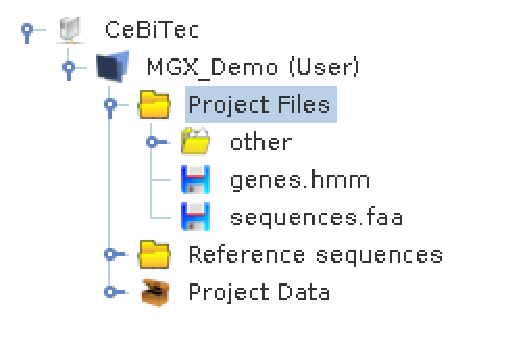
\includegraphics[width=.45\textwidth]{img/mgx/serverfs}
\caption[File storage]{Each project includes flat storage where custom
data can be stored, e.g. own FASTA files to be used as reference databases
for metagenome analysis.}
\label{serverfs}
\end{figure}

While it may be necessary to implement an own pipeline depending on the
desired kind of analysis, the MGX repository hosts predefined pipeline
templates addressing the most common cases: The ``BestHit-Blast'' template
can be used to annotate metagenome sequences with the description of a
Blast hit after the user has uploaded a FASTA file containing amino acid
sequences, and the ``BestHit-HMM'' template provides the same functionality
for hidden Markov models (HMMs).


\section{Reference mapping}

\subsection{Importing reference genomes}

MGX provides several analysis pipelines to align metagenome reads to reference genomes;
before these pipelines can be used, the corresponding reference genome has to be added
to the project. There are two possible ways to achieve this: The MGX repository hosts
published and annotated reference genomes obtained from the NCBI; in addition, users
may choose to upload a custom reference sequence in FASTA, GenBank or EMBL format, e.g.
a finished but unpublished genome not available from official sources.\\

\begin{figure}[H]
\centering
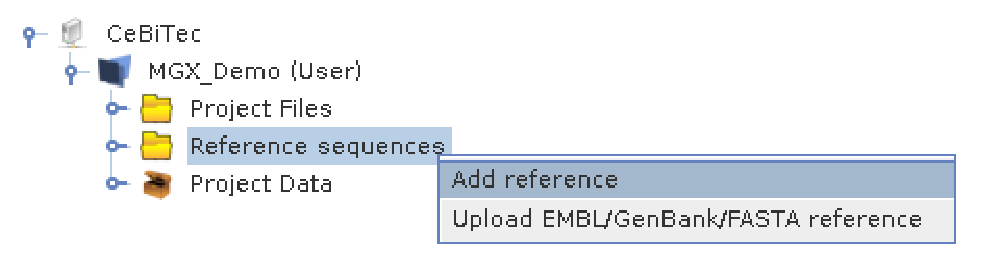
\includegraphics[width=.9\textwidth]{img/mgx/addReference}
\caption[Reference import]{Reference sequences to be used as mapping targets may be
imported from the global repository or uploaded in EMBL/GenBank/FASTA format.}
\label{addref}
\end{figure}

To add a reference genome, right-click on the ``Reference sequences'' node within the
project view and select either ``Add reference'' to access the MGX repository or
``Upload EMBL/GenBank/FASTA reference'' to provide an own sequence (\ref{addref}).\\

Once the import is complete, the reference genome is available for analysis and
can be selected for the corresponding analysis pipelines which provide reference
mapping, e.g. BowTie or FR-HIT.

\subsection{Displaying reference mappings}

\begin{figure}[H]
\centering
\includegraphics[width=\textwidth]{img/mgx/RefMapping}
\caption[Reference mapping]{The reference mapping component showing alignment results for a metatranscriptome dataset mapped to the reference genome of one of the dominant organisms. From top to bottom, the component displays a) navigation and coverage histogram, b) currently selected interval and c) aligned DNA sequences for the interval. Color coding refers to relative sequence identity.}
\label{refmap}
\end{figure}

\begin{figure}[H]
\centering
\includegraphics[width=\textwidth]{img/mgx/FragRecruitment}
\caption[Fragment recruitment]{An alternate visualization mode is the generation of fragment recruitment plots, here showing the
same data as described previously (\ref{refmap}). The view mode features the fragment recruitment plot itself and additionally
provides stacked bars summarizing mapping identity within reference intervals, grouped into low (red), medium (yellow, $\ge$ 75\%) and
high (green, $\ge$ 97\%) quality mappings.}
\label{fragrec}
\end{figure}


Alignment of metagenome or metatranscriptome data to reference sequences of known origin allows researchers to evaluate
relative identity between metagenome sequences and the actual strain or to obtain an overview of gene expression within
a meta-transcriptome. MGX currently provides predefined pipelines employing BLAST \cite{BLAST}, FR-HIT \cite{FRHIT} and Bowtie 2 \cite{BOWTIE}.
The reference mapping component is provided to inspect and browse alignment results, offering both a generic alignment view
where each mapped sequence is colored according to mapping identity, as well as a fragment recruitment view. Switching between
view modes is possible from the context menu of the mapping component.

\section{Search}

\begin{figure}[H]
\centering
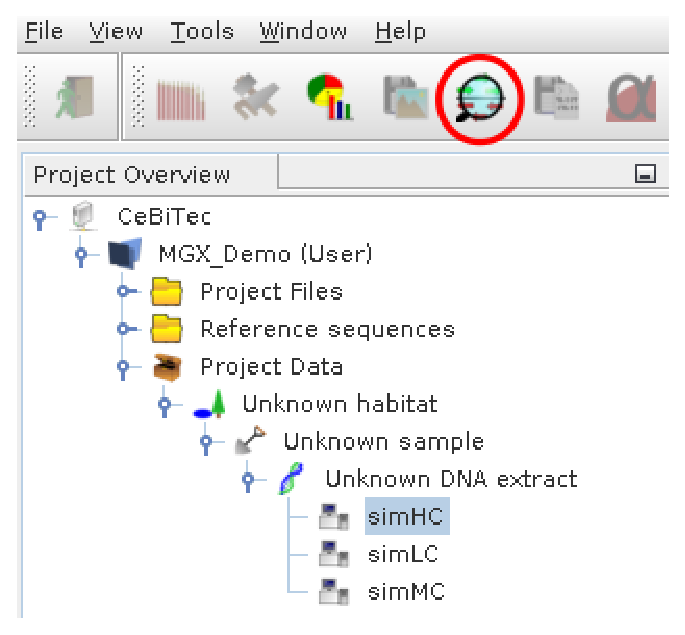
\includegraphics[width=.5\textwidth]{img/mgx/SearchOpen}
\caption[Metagenome search]{Icon for the metagenome search component.}
\label{search1}
\end{figure}

\begin{figure}[H]
\centering
\includegraphics[width=.9\textwidth]{img/mgx/SearchTC}
\caption[Metagenome search]{Search component showing results for the term ``polymeras''. The search was performed
within the select metagenomes simHC and simLC (top left); the bottom part shows an individual sequence identified
by the search. Search results are displayed together with all other attributes available for a sequences, thus allowing
to identify co-occurence of results.}
\label{search2}
\end{figure}

